\documentclass[12pt,a4paper]{article}
\usepackage[utf8]{inputenc}

\usepackage{amsmath}
\usepackage{amsfonts}
\usepackage{amssymb}
\usepackage{graphicx}
\usepackage{listings}
\usepackage[margin=1.0in]{geometry}
\usepackage{caption}
\usepackage{subcaption}
\usepackage{float}
\usepackage[utf8]{inputenc}
\usepackage{refstyle}
\usepackage{spverbatim}
\usepackage{listings}
\usepackage{csvsimple}
\usepackage{adjustbox}
\usepackage{cancel}
\usepackage{scalerel,stackengine}
\stackMath
\newcommand\reallywidehat[1]{%
\savestack{\tmpbox}{\stretchto{%
  \scaleto{%
    \scalerel*[\widthof{\ensuremath{#1}}]{\kern-.6pt\bigwedge\kern-.6pt}%
    {\rule[-\textheight/2]{1ex}{\textheight}}%WIDTH-LIMITED BIG WEDGE
  }{\textheight}% 
}{0.5ex}}%
\stackon[1pt]{#1}{\tmpbox}%
}
\parskip 1ex

\lstset{numbers=left,
	title=\lstname,
	numberstyle=\tiny, 
	breaklines=true,
	tabsize=4,
	language=Python,
	morekeywords={with,super,as},,
	frame=single,
	basicstyle=\footnotesize\tt,
	commentstyle=\color{comment},
	keywordstyle=\color{keyword},
	stringstyle=\color{string},
	backgroundcolor=\color{background},
	showstringspaces=false,
	numbers=left,
	numbersep=5pt,
	literate=
		{æ}{{\ae}}1
		{å}{{\aa}}1
		{ø}{{\o}}1
		{Æ}{{\AE}}1
		{Å}{{\AA}}1
		{Ø}{{\O}}1
	}

\usepackage{bm}
\PassOptionsToPackage{hyphens}{url}\usepackage{hyperref}
\usepackage[usenames, dvipsnames]{color}

\begin{document}

\begin{center}
\LARGE{\textbf{Project 2: Classification and Regression, from linear and logistic regression to neural networks}}
\\
\large{\textbf{Course: FYS-STK4155}}
\\
\large{\textbf{Semester: Autumn 2020}}
\\
\large{\textbf{Name: Sander Losnedahl}}
\end{center}

\begin{center}
\Large{\textbf{Abstract}}
\end{center}

\noindent a

\newpage

\begin{center}
\Large{\textbf{Introduction}}
\end{center}

\noindent a

\newpage

\begin{center}
\Large{\textbf{Preliminaries}}
\end{center}

\noindent a

\newpage

\begin{center}
\Large{\textbf{Exercise 1a): a}}
\end{center}

\begin{center}
\large{\textbf{Defining the heat equation}}
\end{center}

\noindent In this exercise we want to mathematically describe how heat can transfer within a rod of length L over a given time interval t. The rod will initially be heated at time $t = 0$ and the heat will decay after this time. How the heat changes as function of time and space is given by the heat equation as seen below.

\begin{equation}\label{eq:heatEquation}
\frac{\partial u(x,t)}{\partial t} = \frac{K_0}{c\rho} \frac{\partial^2 u(x,t)}{\partial x^2} 
\end{equation}

\noindent where $u(x,t)$ is the temperature at a specific time t and a position x. The term $\frac{K_0}{c\rho}$ is the thermal diffusivity which consists of thermal conductivity $K_0$ divided by the specific heat capacity c times the density of the material $\rho$. This quantity is a measure of the rate of heat transfer from the heated part of the rod to the cold part of the rod. 
\\
Equation \ref{eq:heatEquation} is a partial differential equation (PDE) which means that we need an initial condition and two boundary conditions in order to solve the equation. The initial condition can be interpreted as how much the rod is heated at $t = 0$ while the boundary conditions can be interpreted as how the heat reacts to the ends of the rod at $x = 0$ and $x = L$. The boundary conditions in this case is given by equations \ref{eq:boundary0} and \ref{eq:boundaryL}.

\begin{equation}\label{eq:boundary0}
u(0,t) = 0
\end{equation}

\begin{equation}\label{eq:boundaryL}
u(L,t) = 0
\end{equation}

\noindent We can set the initial condition such that the rod is heated the most at the middle of the rod and least at the end of the road. Such a condition can be described by a sine function as given in equation \ref{eq:initial}.

\begin{equation}\label{eq:initial}
u(x,0) = sin(\pi x)
\end{equation}

\noindent One can observe from equation \ref{eq:initial} that a rod of length 1 is heated the most at $0.5$ and is not heated at all at the ends of the rod. 

\begin{center}
\large{\textbf{Analytical solution to the heat equation}}
\end{center}

\noindent We can now split equation \ref{eq:heatEquation} into its spatial and temporal components such that 

\begin{equation}\label{eq:split}
u(x,t) = X(x)T(t)
\end{equation}

\noindent Equation \ref{eq:split} can then be solved for x and t respectively. We start by taking the partial derivatives of equation \ref{eq:split} with respect to both t and x.

\begin{equation}\label{eq:split2}
\begin{aligned}
u_t = X(x)T'(t)
\\
u_{xx} = X''(x)T(t)
\end{aligned}
\end{equation}

\noindent Equation \ref{eq:heatEquation} then takes the form

\begin{equation}\label{eq:heatSplit}
\begin{aligned}
u_t = u_{xx}
\\
X(x)T'(t) = X''(x)T(t)
\\
\frac{X''(x)}{X(x)} = \frac{T'(t)}{T(t)} = \lambda
\end{aligned}
\end{equation}

\noindent where $\lambda$ is some constant. We can first solve equation \ref{eq:heatSplit} for its spatial part X such that

\begin{equation}\label{eq:solveX}
\begin{aligned}
\frac{X''(x)}{X(x)} = \lambda
\\
X''(x) - \lambda X(x) = 0
\end{aligned}
\end{equation}

\noindent Equation \ref{eq:solveX} is recognized as a Sturm-Liouville problem when $\lambda$ represents the eigenvalues of equation \ref{eq:solveX} (Hancock, 2006). This means that the solutions to equation \ref{eq:solveX} is given by equation \ref{eq:eigenSol}.

\begin{equation}\label{eq:eigenSol}
X_n(x)= b_n sin(n\pi x)
\end{equation}

\noindent where n is an eigenfunction given by $n = \sqrt{\lambda}/\pi$ where $\lambda$ are the eigenvalues of the Sturm-Liouville problem. Solutions then arise at $\lambda = \pi^2 n^2$ and from equation \ref{eq:heatSplit} the solution with respect to $T'(t)$ is found.

\begin{equation}\label{eq:eigenSolT}
\begin{aligned}
\frac{T'(t)}{T(t)} = \lambda
\\
T'(t) = \lambda T(t)
\end{aligned}
\end{equation}

\noindent which has the solution

\begin{equation}\label{eq:realSolT}
T'(t) = e^{\pi^2 n^2 t}
\end{equation}

\noindent We can then find the solution for $u(x,t)$ by combining equation \ref{eq:eigenSol} and equation \ref{eq:realSolT} such that

\begin{equation}\label{eq:heatsol}
u_n(x,t) = b_n sin(n\pi x)e^{\pi^2 n^2 t}
\end{equation}

\noindent The subscript n denotes the individual eigenfunctions that solve the heat equation, however, most of them do not satisfy the initial condition in equation \ref{eq:initial}. The sum of these functions may satisfy the initial condition and thus, equation \ref{eq:heatsol} becomes

\begin{equation}\label{eq:sumN}
u_n(x,t) = \sum_{n=1}^{\infty} b_n sin(n\pi x)e^{\pi^2 n^2 t}
\end{equation}

\noindent One can observe from equation \ref{eq:sumN} that the exponential term decreases as n increases. Therefore, a reasonable approximation may be to only utilize the first term of the sum such that equation \ref{eq:sumN} can be written as

\begin{equation}\label{eq:finalSol}
u_n(x,t) = sin(\pi x)e^{\pi^2 t}
\end{equation}

\noindent where the constant $b_n$ has been set to one. This is the final solution of the heat equation that will be implemented in the code.

\newpage

\begin{center}
\Large{\textbf{Exercise 1b: A numerical approach to solving the heat equation}}
\end{center}

\begin{center}
\large{\textbf{The forward Euler approach}}
\end{center}

\noindent The heat equation is a partial differential equation that can be solved numerically using the forward Euler algorithm (sometimes referred to as the explicit Euler method). This algorithm aims to incrementally approximate the gradient of spatial and temporal parts of the heat equation by utilizing the definition of the derivative as seen in equations \ref{eq:gradT} and \ref{eq:gradx}.

\begin{equation}\label{eq:gradT}
u_t \approx \frac{u(x, t+\Delta t) - u(x,t)}{\Delta t}
\end{equation}

\begin{equation}\label{eq:gradx}
u_{xx} \approx \frac{u(x + \Delta x, t) - 2u(x,t) + u(x-\Delta x,t)}{\Delta x^2}
\end{equation}

\noindent where $\Delta$ represents the incremental step size in space or time. Since the initial conditions are known, the forward Euler algorithm can incrementally approximate the change in heat from the middle of the rod and out towards the boundary. Equations \ref{eq:gradT} and \ref{eq:gradx} can be combined using the heat equation from equation \ref{eq:heatEquation} such that

\begin{equation}\label{eq:forwardEuler1}
\begin{aligned}
u_t = u_{xx}
\\
\frac{u(x,t+\Delta t) - u(x,t)}{\Delta t} = \frac{u(x+\Delta x, t)-2u(x,t)+u(x-\Delta x,t)}{\Delta x^2}
\\
\frac{u_j^{n+1}-u_j^n}{\Delta t} = \frac{u_{j+1}^n - 2u_j^n + u_{j-1}^2}{\Delta x^2}
\end{aligned}
\end{equation}

\noindent where the subscript j denotes the step in space and the subscript n denotes the step in time. We can solve equation \ref{eq:forwardEuler1} for $u_j^{n+1}$ such that we can calculate the heat incrementally forward in time. Thus, equation \ref{eq:forwardEuler1} becomes

\begin{equation}\label{eq:forwardEuler2}
\begin{aligned}
u_j^{n+1} = \Delta t(\frac{u_{j+1}^n - 2u_j^n + u_{j-1}^2}{\Delta x^2})+u_j^n
\\
u_j^{n+1} = (1-2\frac{\Delta t}{\Delta x^2})u_j^n + \frac{\Delta t}{\Delta x^2}(u_{j+1}^n + u_{j-1}^n)
\end{aligned}
\end{equation}

\noindent Equation \ref{eq:forwardEuler2} is only stable for $\frac{\Delta t}{\Delta x^2} \leq 0.5$, so the implementation needs to adjust $\Delta t$ according to $\Delta x$. The implementation of equation \ref{eq:forwardEuler2} allows us to solve the heat equation incrementally and the results are then compared to the analytical solution in the following section.

\begin{center}
\large{\textbf{Comparing the analytical and numerical solutions of the heat equation}}
\end{center}

\noindent We now compare how the heat translates throughout the rod at a given time for both the analytical implementation and for the forward Euler implementation. It was found that the heat decayed quickly. Therefore, good time intervals of observing the heat was found to be at $t = 0$ (initial heat), $t = 0.5$ and $t = 1$. Figures \ref{fig:rodHeatEulerT0DX01}, \ref{fig:rodHeatEulerT05DX01} and \ref{fig:rodHeatEulerT1DX01} shows the heat distribution in the rod at these given times for $\Delta t = 0.005$ and $\Delta x = 0.1$ for both the analytical and forward Euler implementations (and their difference).

\begin{figure}[H]
\centering
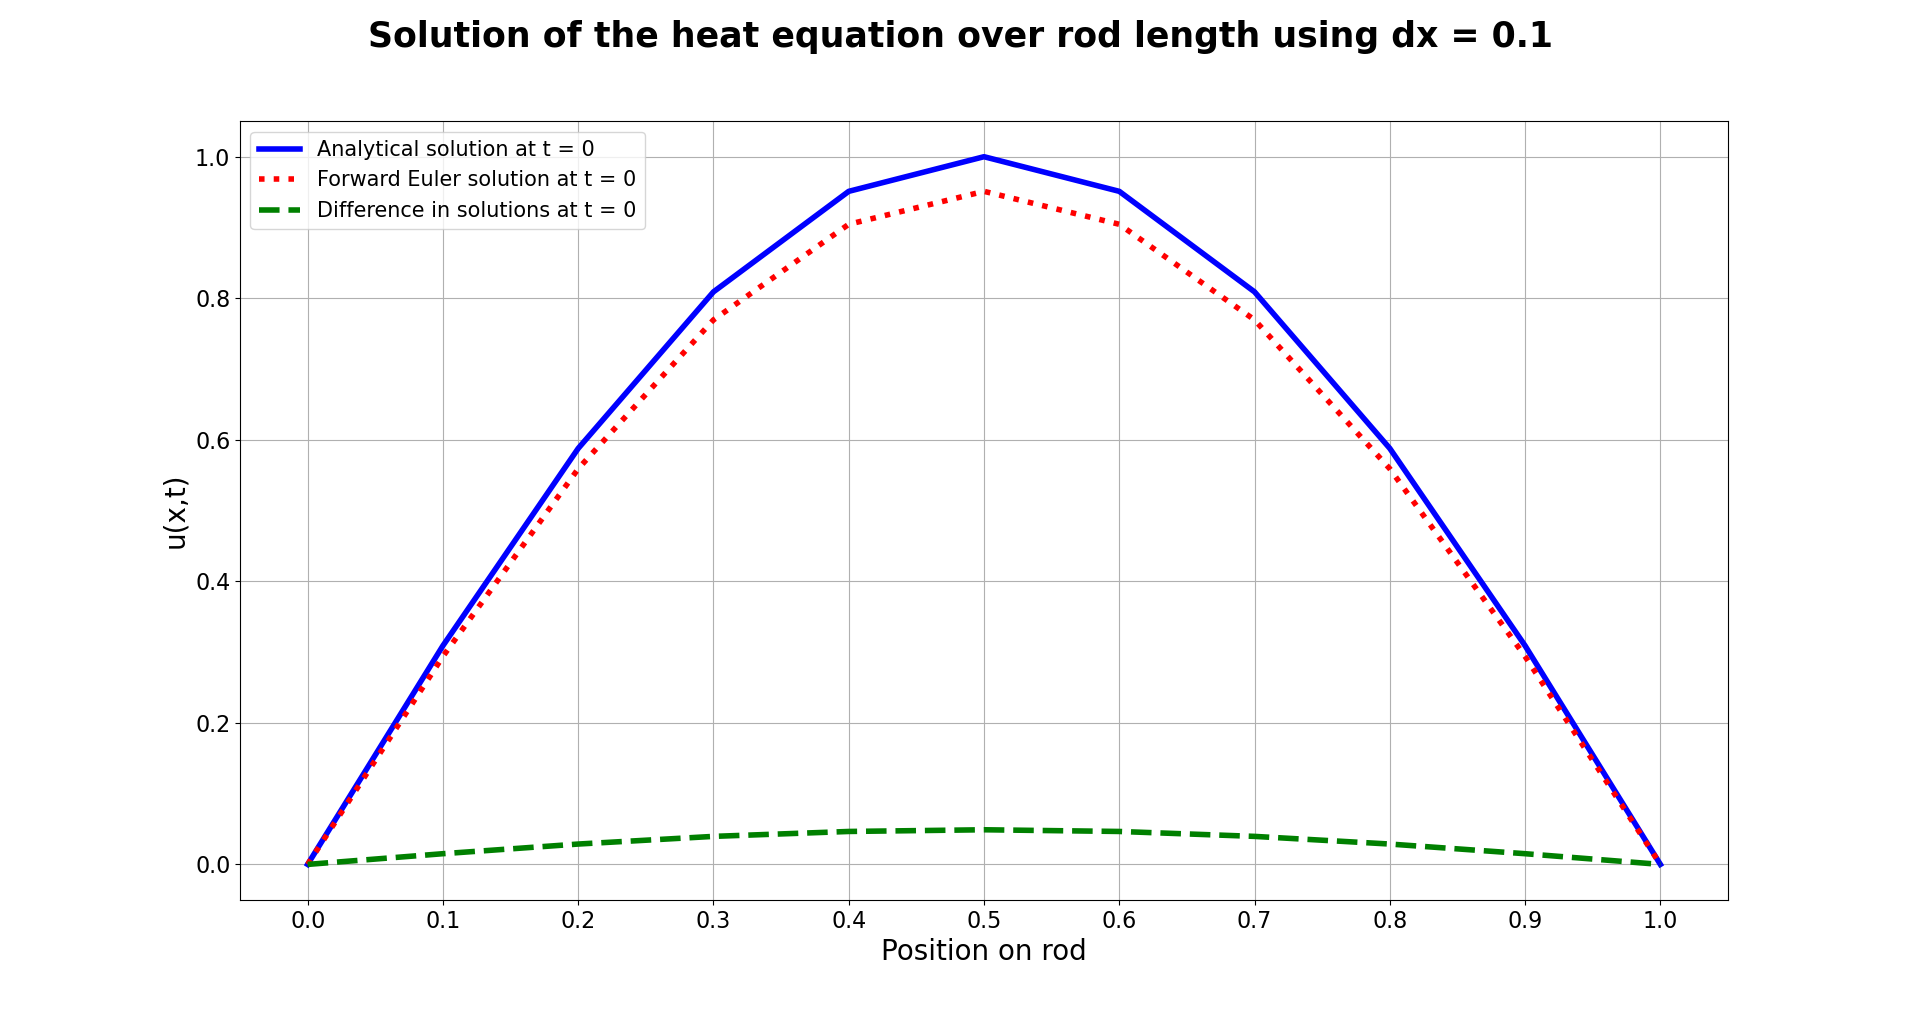
\includegraphics[width = 1\linewidth]{C:/Users/Sander/Documents/GitHub/FYS-STK4155/Project3/Report/Figures/Heat_Euler_t0_dx01.PNG}
\caption{\label{fig:rodHeatEulerT0DX01} Heat distribution within the rod for both analytical (blue) and forward Euler implementations (red). The heat is measured at $t = 0$ using step sizes of $\Delta t = 0.005$ and $\Delta x = 0.1$.}
\end{figure}

\begin{figure}[H]
\centering
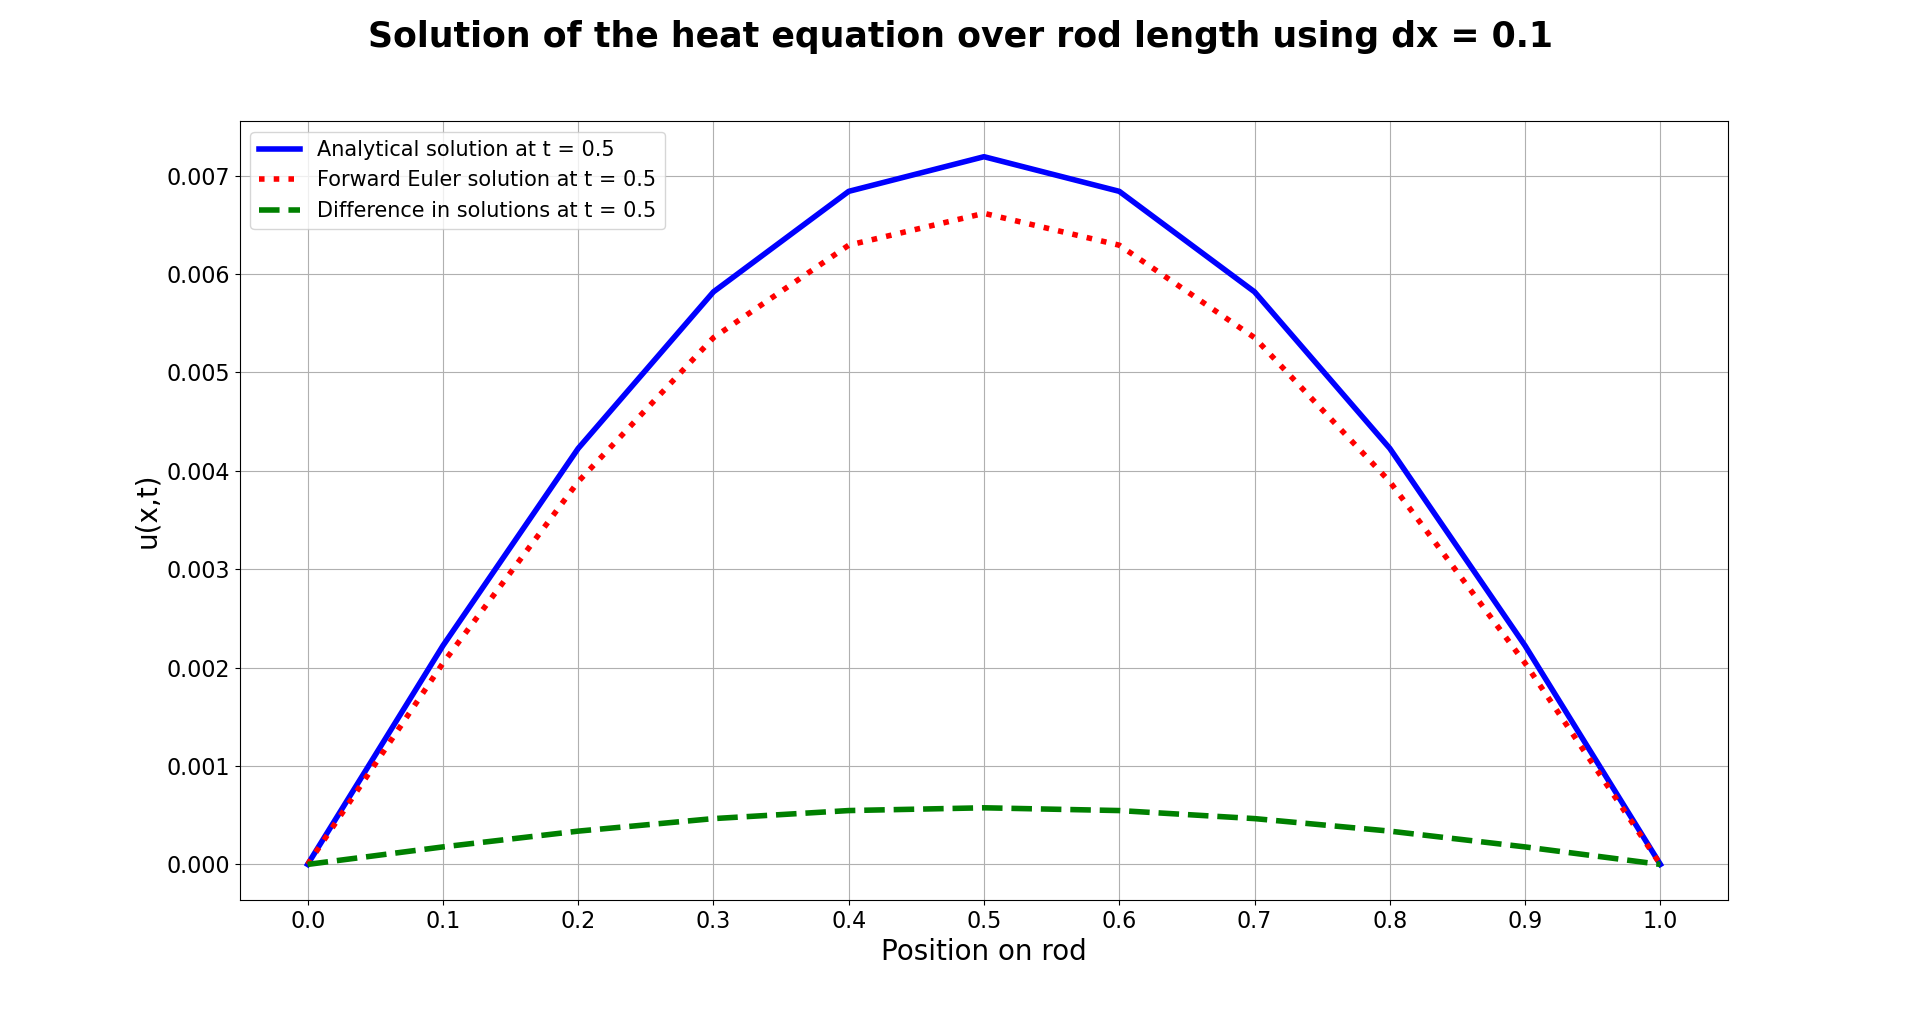
\includegraphics[width = 1\linewidth]{C:/Users/Sander/Documents/GitHub/FYS-STK4155/Project3/Report/Figures/Heat_Euler_t05_dx01.PNG}
\caption{\label{fig:rodHeatEulerT05DX01} Heat distribution within the rod for both analytical (blue) and forward Euler implementations (red). The heat is measured at $t = 0.5$ using step sizes of $\Delta t = 0.005$ and $\Delta x = 0.1$.}
\end{figure}

\begin{figure}[H]
\centering
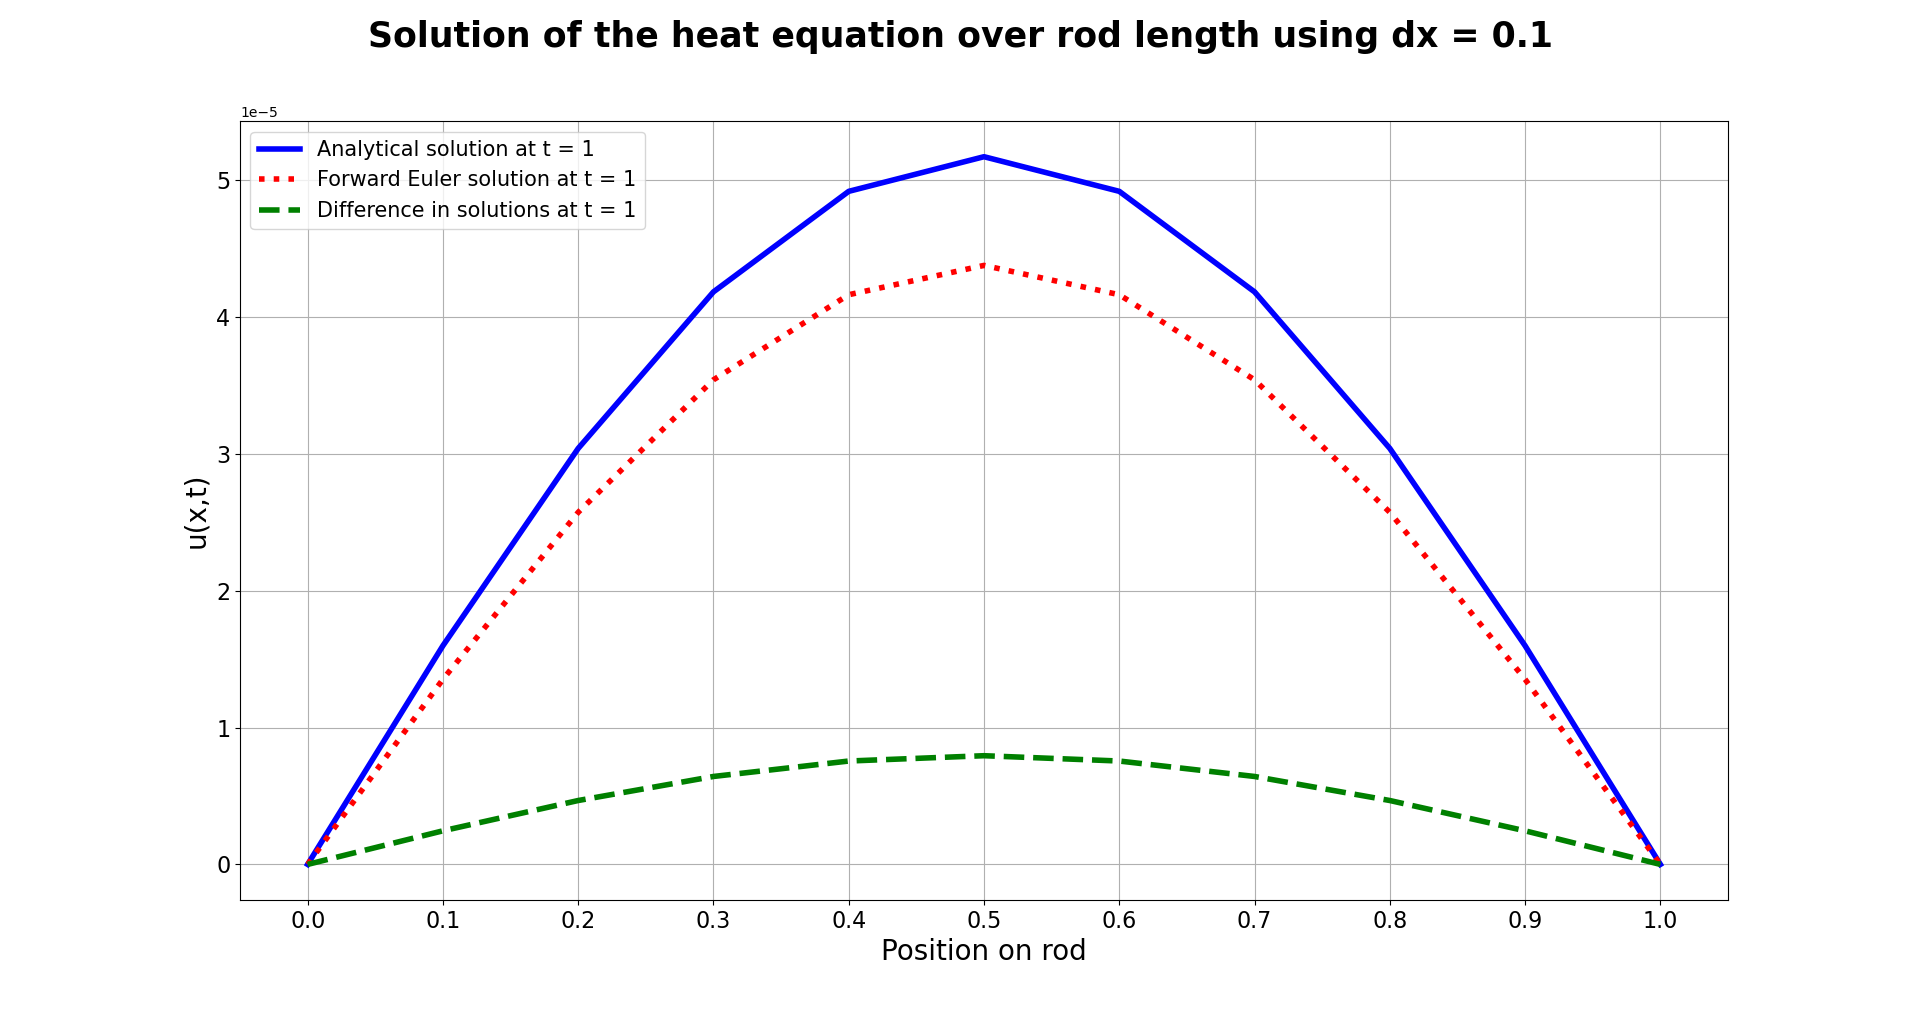
\includegraphics[width = 1\linewidth]{C:/Users/Sander/Documents/GitHub/FYS-STK4155/Project3/Report/Figures/Heat_Euler_t1_dx01.PNG}
\caption{\label{fig:rodHeatEulerT1DX01} Heat distribution within the rod for both analytical (blue) and forward Euler implementations (red). The heat is measured at $t = 1$ using step sizes of $\Delta t = 0.005$ and $\Delta x = 0.1$.}
\end{figure}

\noindent One first observed that the rod is heated the most at the middle $x = 0.5$, which is according to the initial condition of equation \ref{eq:initial}. One can also observe that the forward Euler lies pretty close to the analytical solution. The difference between the analytical solution and the forward Euler solution decreases as time increases (the y-axis becomes smaller, so don't get fooled). Additionally, one can observe that the heat decays fairly quickly as most of the heat is gone within 1 second. 
\\
We now decrease the step size in space from $\Delta x = 0.1$ to $\Delta x = 0.01$, and this means further we need to adjust the step size in time according to $\frac{\Delta t}{\Delta x^2} \leq 0.5$. Therefore, the new step size in time becomes $\Delta t = 0.5*0.01^2 = 0.00005$. Figures \ref{fig:rodHeatEulerT0DX001}, \ref{fig:rodHeatEulerT05DX001} and \ref{fig:rodHeatEulerT1DX001} shows the same as the above figures, but using the new step sizes.

\begin{figure}[H]
\centering
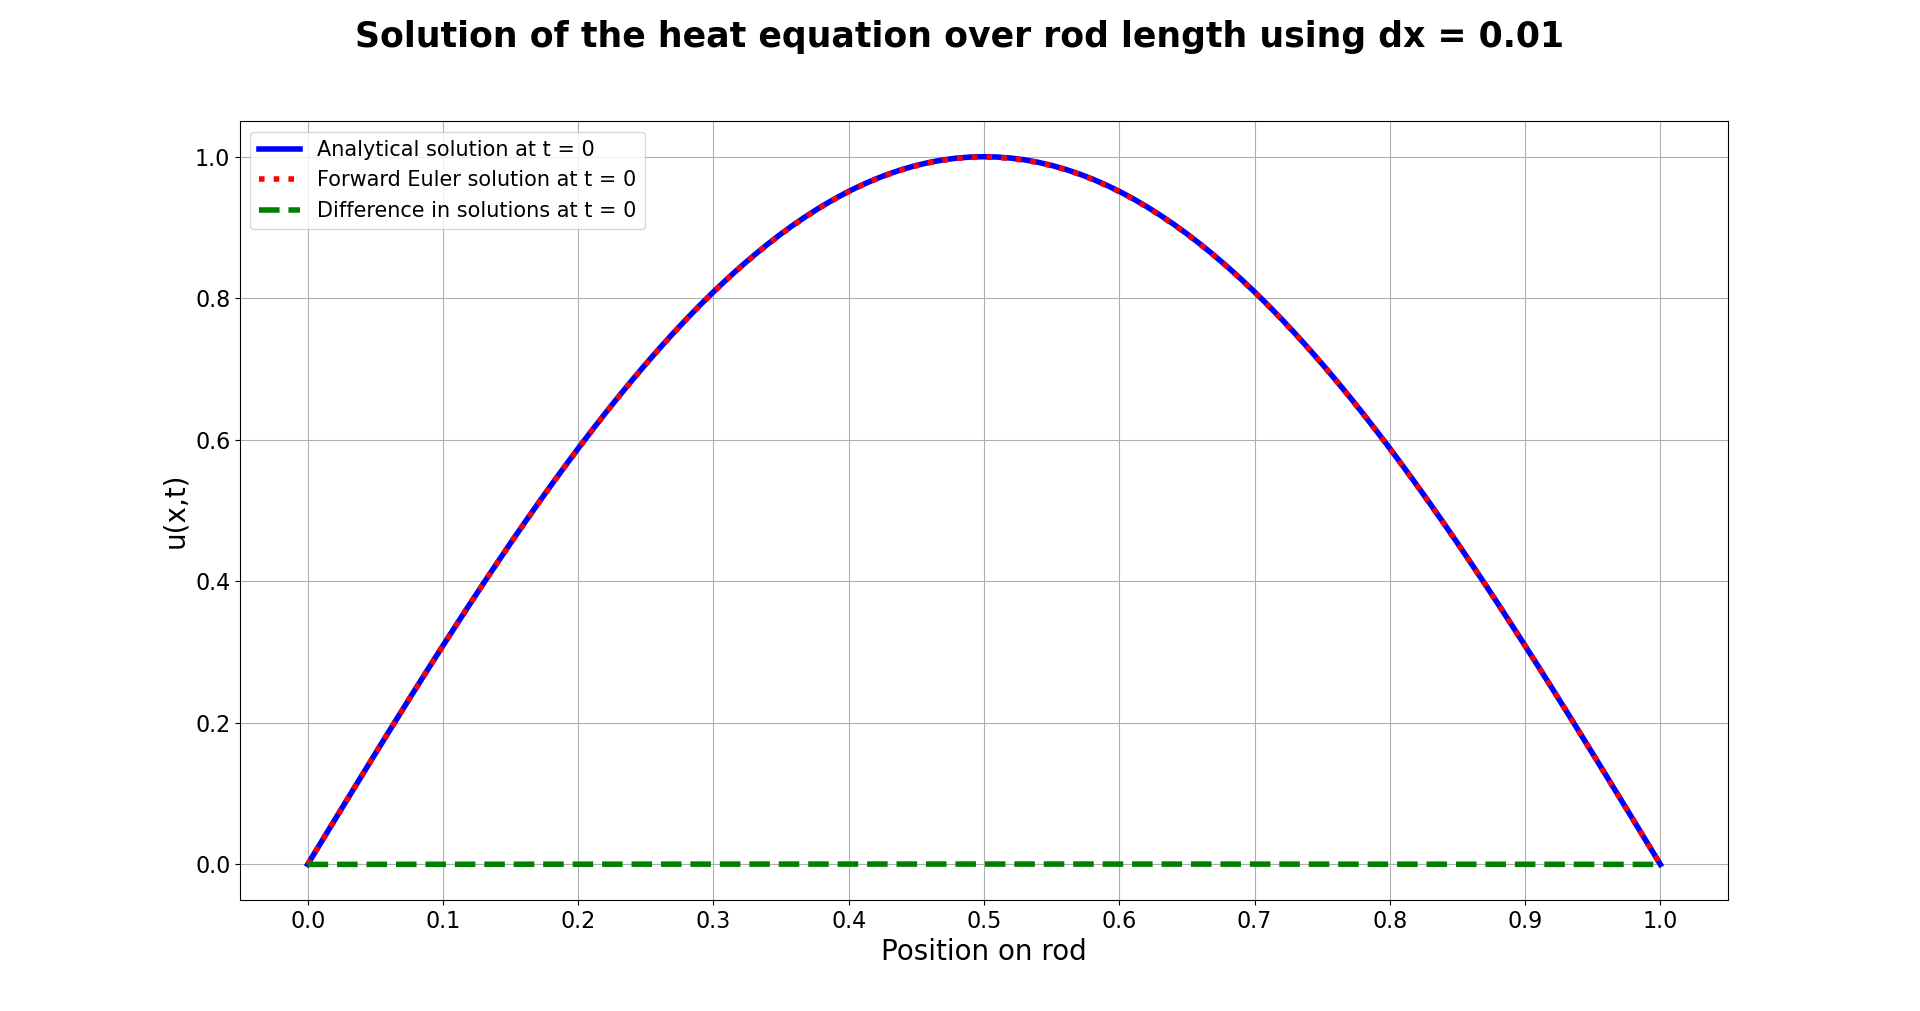
\includegraphics[width = 1\linewidth]{C:/Users/Sander/Documents/GitHub/FYS-STK4155/Project3/Report/Figures/Heat_Euler_t0_dx001.PNG}
\caption{\label{fig:rodHeatEulerT0DX001} Heat distribution within the rod for both analytical (blue) and forward Euler implementations (red). The heat is measured at $t = 0$ using step sizes of $\Delta t = 0.00005$ and $\Delta x = 0.01$.}
\end{figure}

\begin{figure}[H]
\centering
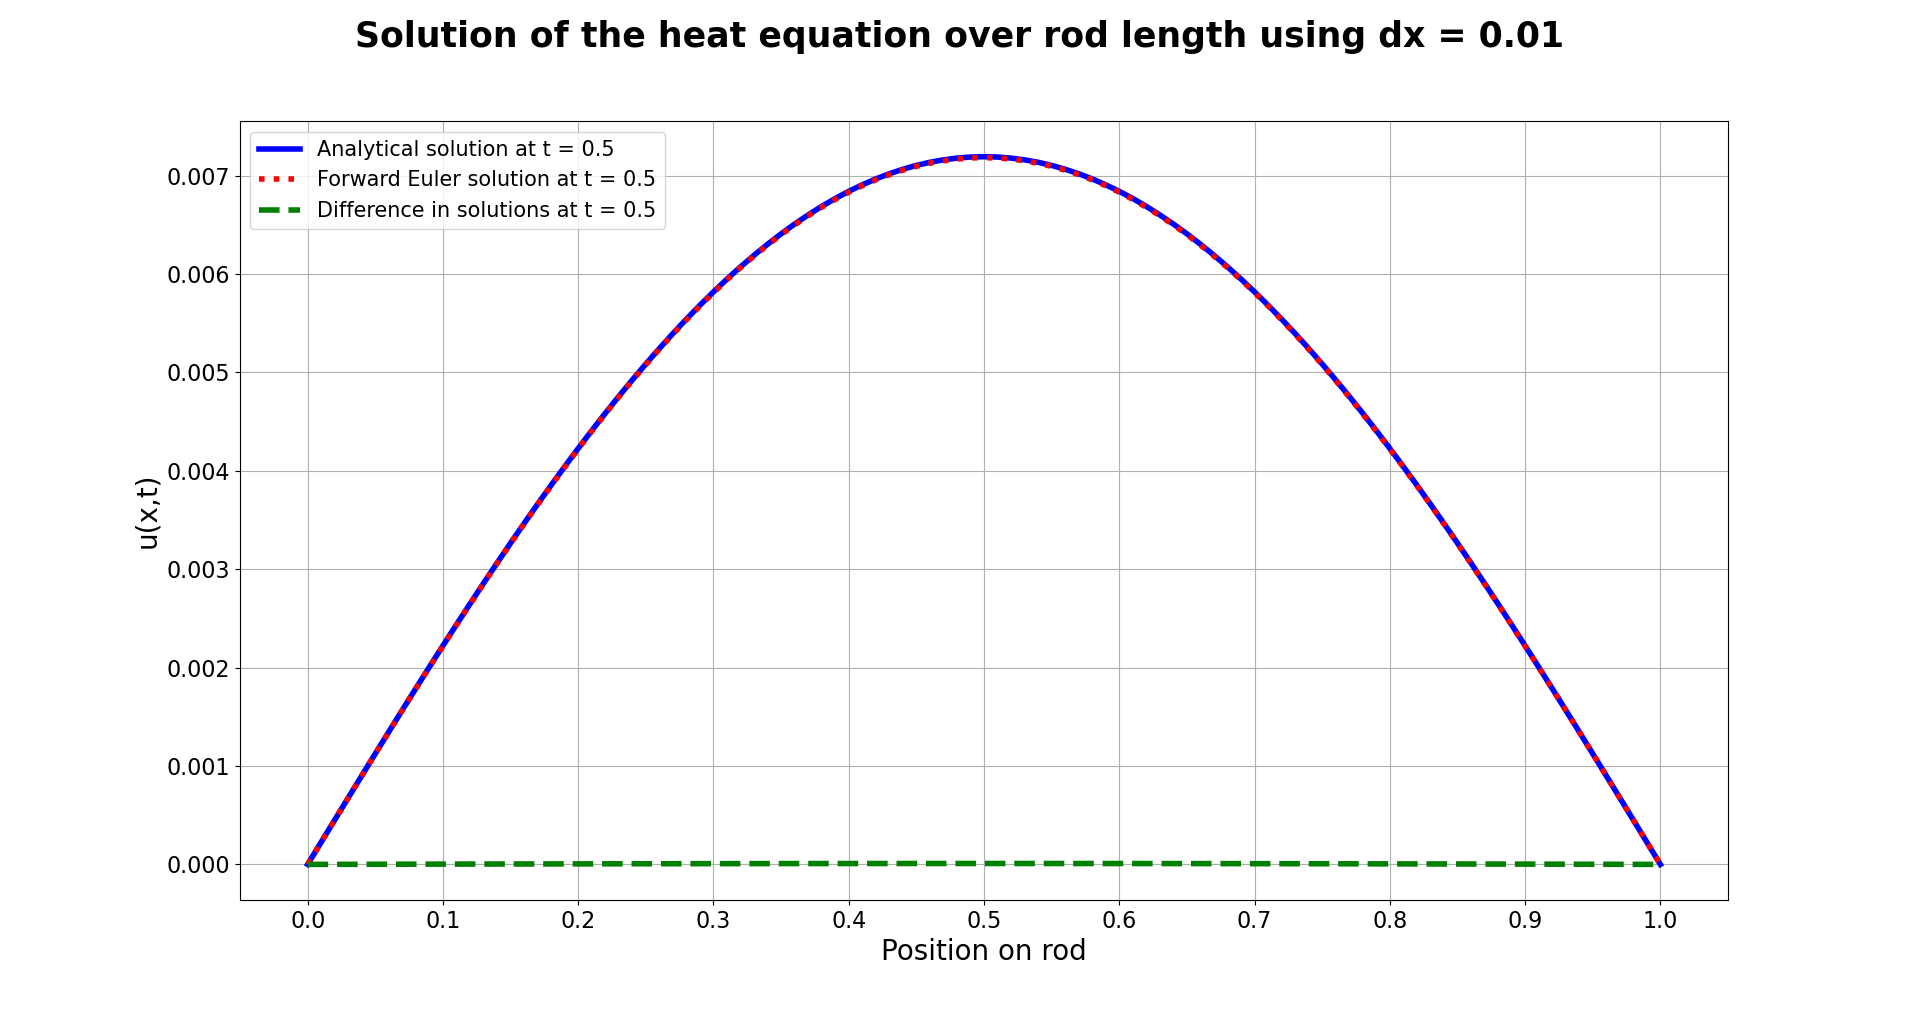
\includegraphics[width = 1\linewidth]{C:/Users/Sander/Documents/GitHub/FYS-STK4155/Project3/Report/Figures/Heat_Euler_t05_dx001.PNG}
\caption{\label{fig:rodHeatEulerT05DX001} Heat distribution within the rod for both analytical (blue) and forward Euler implementations (red). The heat is measured at $t = 0.5$ using step sizes of $\Delta t = 0.00005$ and $\Delta x = 0.01$.}
\end{figure}

\begin{figure}[H]
\centering
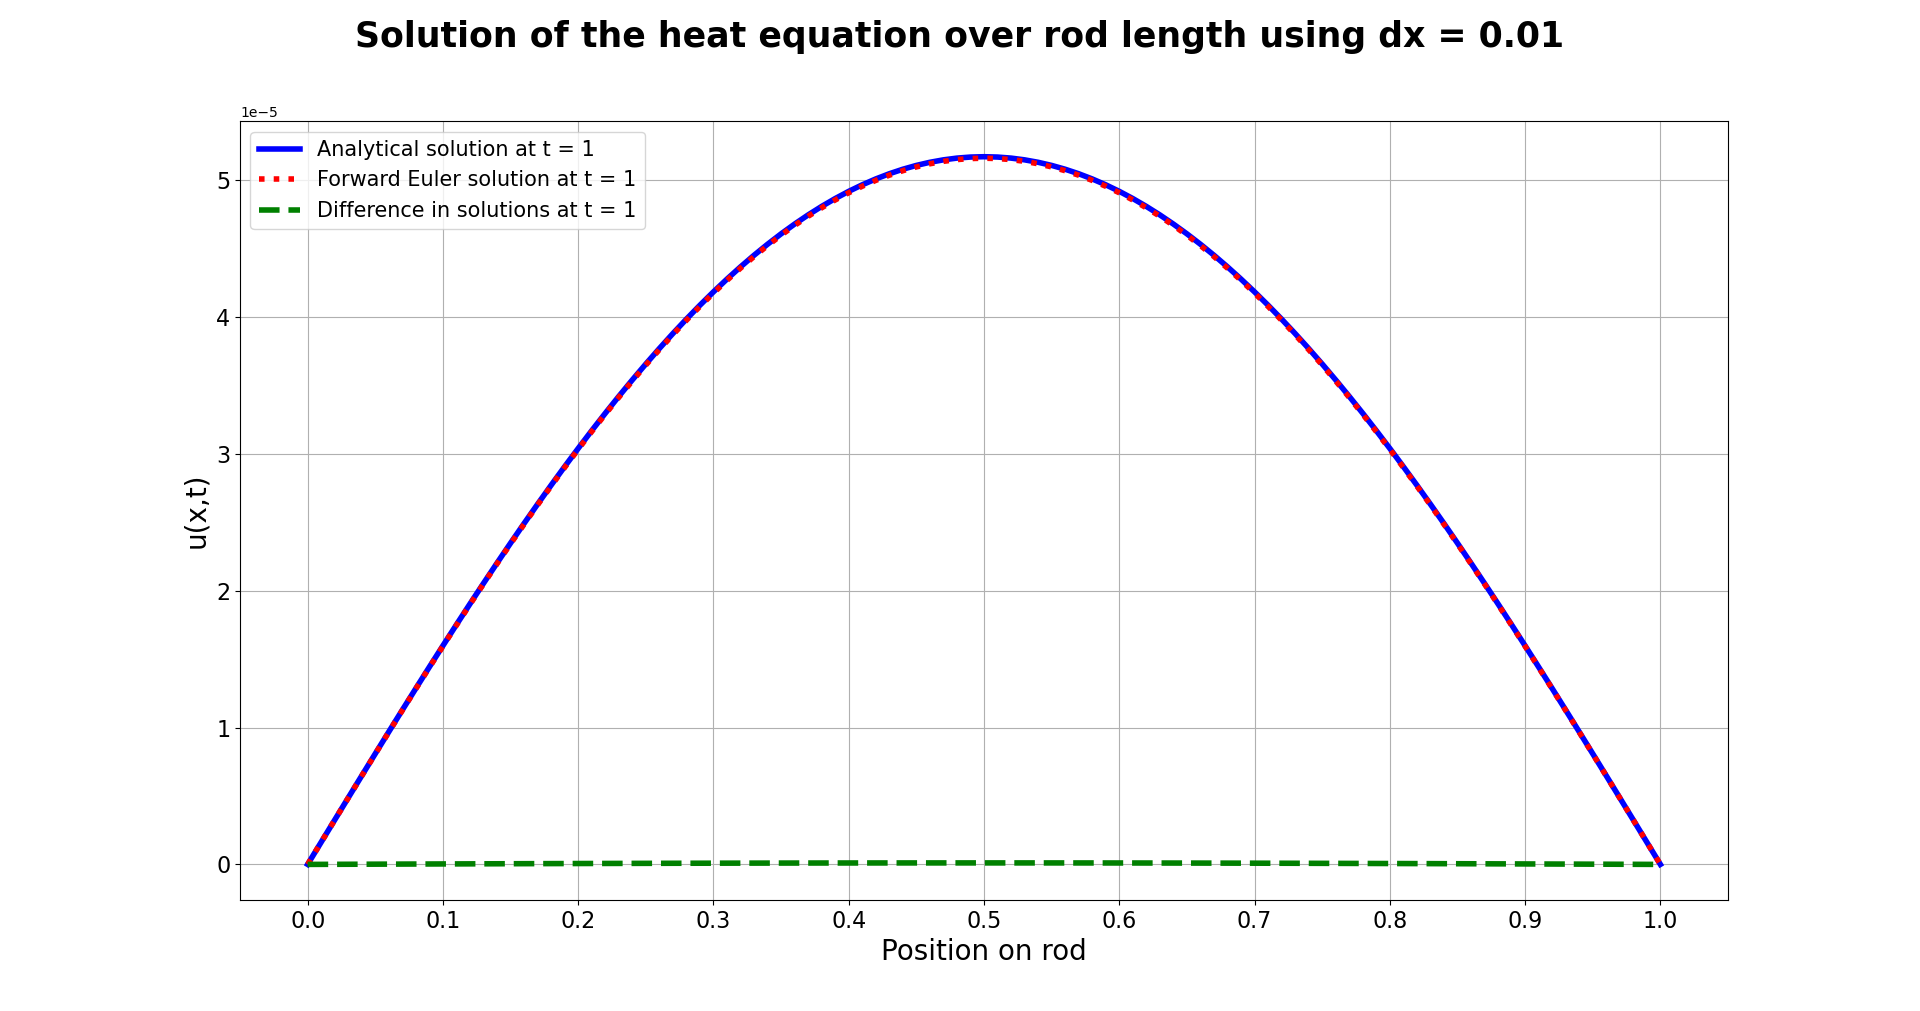
\includegraphics[width = 1\linewidth]{C:/Users/Sander/Documents/GitHub/FYS-STK4155/Project3/Report/Figures/Heat_Euler_t1_dx001.PNG}
\caption{\label{fig:rodHeatEulerT1DX001} Heat distribution within the rod for both analytical (blue) and forward Euler implementations (red). The heat is measured at $t = 1$ using step sizes of $\Delta t = 0.00005$ and $\Delta x = 0.01$.}
\end{figure}

\noindent It is now observed that the forward Euler implementation matches the analytical implementation perfectly at all times. The reason for this is because the definition of the derivative in which the forward Euler relies on is a better approximation when the step sizes are small. This means further that the forward Euler implementation can accurately represent the heat distribution within a rod at all times and places.

\newpage

\begin{center}
\Large{\textbf{Exercise c): Solving PDEs with deep neural networks}}
\end{center}

\begin{center}
\large{\textbf{Neural network implementation}}
\end{center}

\noindent The concepts and details of a neural network was discussed in Project 2 which can be found at \href{{https://github.com/sanderwl/FYS-STK4155/tree/master/Project2/Project2}}{\nolinkurl{https://github.com/sanderwl/FYS-STK4155/tree/master/Project2/Project2}}. Much of the concepts are the same, that is, we pass an input through a network of hidden layers and neurons and an output is the same. However, the implementation is slightly different. 
\\
The neural network still aims to minimize some cost function which is this case is the MSE given by equation \ref{eq:MSE}.

\begin{equation}\label{eq:MSE}
\textrm{MSE} = \frac{1}{n} \sum_{i = 1}^n (\textrm{prediction error})^2
\end{equation}

\noindent Since $\frac{\partial u(x,t)}{\partial t} - \frac{\partial^2 u(x,t)}{\partial x^2} = 0$ solves the heat equation, it can be utilized as the prediction error. Equation \ref{eq:MSE} then becomes

\begin{equation}\label{eq:MSEHeat}
\textrm{MSE} = \frac{1}{n} \sum_{i = 1}^n (\frac{\partial u(x,t)}{\partial t} - \frac{\partial^2 u(x,t)}{\partial x^2})^2
\end{equation}

\noindent Since we now pretend not to know any solution to the heat equation, we can implement a trial solution. A trial solution must meet the boundary conditions (with already known initial condition). This solution is not guaranteed to minimize the cost function in equation \ref{eq:MSEHeat}, in fact, it is rare that such a solution minimize the cost function. Therefore, we can tune the weights of the neural network through gradient descent and update the weights to find different trial solutions. For each update, the cost function should minimize and a more accurate solution to the heat equation is found. The trial solution g used in this project is given by equation QQQ.

\begin{equation}\label{eq:trial}
g = (1-t)*sin(\pi x) + x(1-x)t*\textrm{output}
\end{equation}

\noindent where $sin(\pi x)$ is the initial condition and output is the output from the neural network in which the gradient descent must handle. 
\\
The neural network is then trained by sending the two variables x and t through the network followed by a weight update through gradient descent on the cost function. This process happens many times and the final trial solution should reflect the analytical solution.

\begin{center}
\large{\textbf{My own implementation vs. Tensorflow}}
\end{center}

\noindent A neural network algorithm was implemented from scratch using what I have learned in this course. However, this algorithm proved way too slow and was thus deemed unfit for this exercise as time is limited. Instead, Tensorflow algorithms were implemented as these yielded fast, stable and good results. Additionally, Tensorflow is easy to handle and has a lot of nice features to play around with. In particular, the Tensorflow version of the Adam optimization algorithm proved to yield great results. The Adam optimization algorithm is really a combinations between stochastic gradient descent and RMSprop (Kingma and Ba, 2014). The algorithm is essentially stochastic gradient descent with momentum where a moving average of the gradient is used instead of the entirety of the gradient. Additionally, the Adam algortihm uses adaptive learning rates just like RMSprop. 

\begin{center}
\large{\textbf{Comparing the analytical and neural network solutions of the heat equation}}
\end{center}

\noindent After implementing the above discussed neural network algorithm, we can take the final trial solution and use it to solve the heat equation and compare it with the analytical and forward Euler implementations. First we have to set some parameters for the neural network to work with. These parameters are defined in table \ref{tab:NNparams} below.

\begin{table}[h]
\caption{\label{tab:NNparams} Parameters of the neural network.}
\centering
\begin{tabular}{|c|c|}
\hline
$\Delta$ t & $0.1$\\
\hline
$\Delta$ x & $0.1$\\
\hline
Number of layers & $10$\\
\hline
Number of neurons in each layer & $10$\\
\hline
Number of iterations & $100000$\\
\hline
Initial learning rate & $0.001$\\
\hline
\end{tabular}
\end{table}

\noindent Since we are doing a stochastic gradient descent like algorithm (Adam optimizer) we have to set some initial learning rate. The number of iterations denotes how many times we do the feed forward/back propagation loop. The other parameters were found through trial and error. These parameters could have been optimized like in Project 2, but the results have shown to be good without exact optimization.
\\
We can first plot the entirety of the 3D heat equation solution as done in figures \ref{fig:3dHeatAna} and \ref{fig:3dHeatNN}.

\begin{figure}[H]
\centering
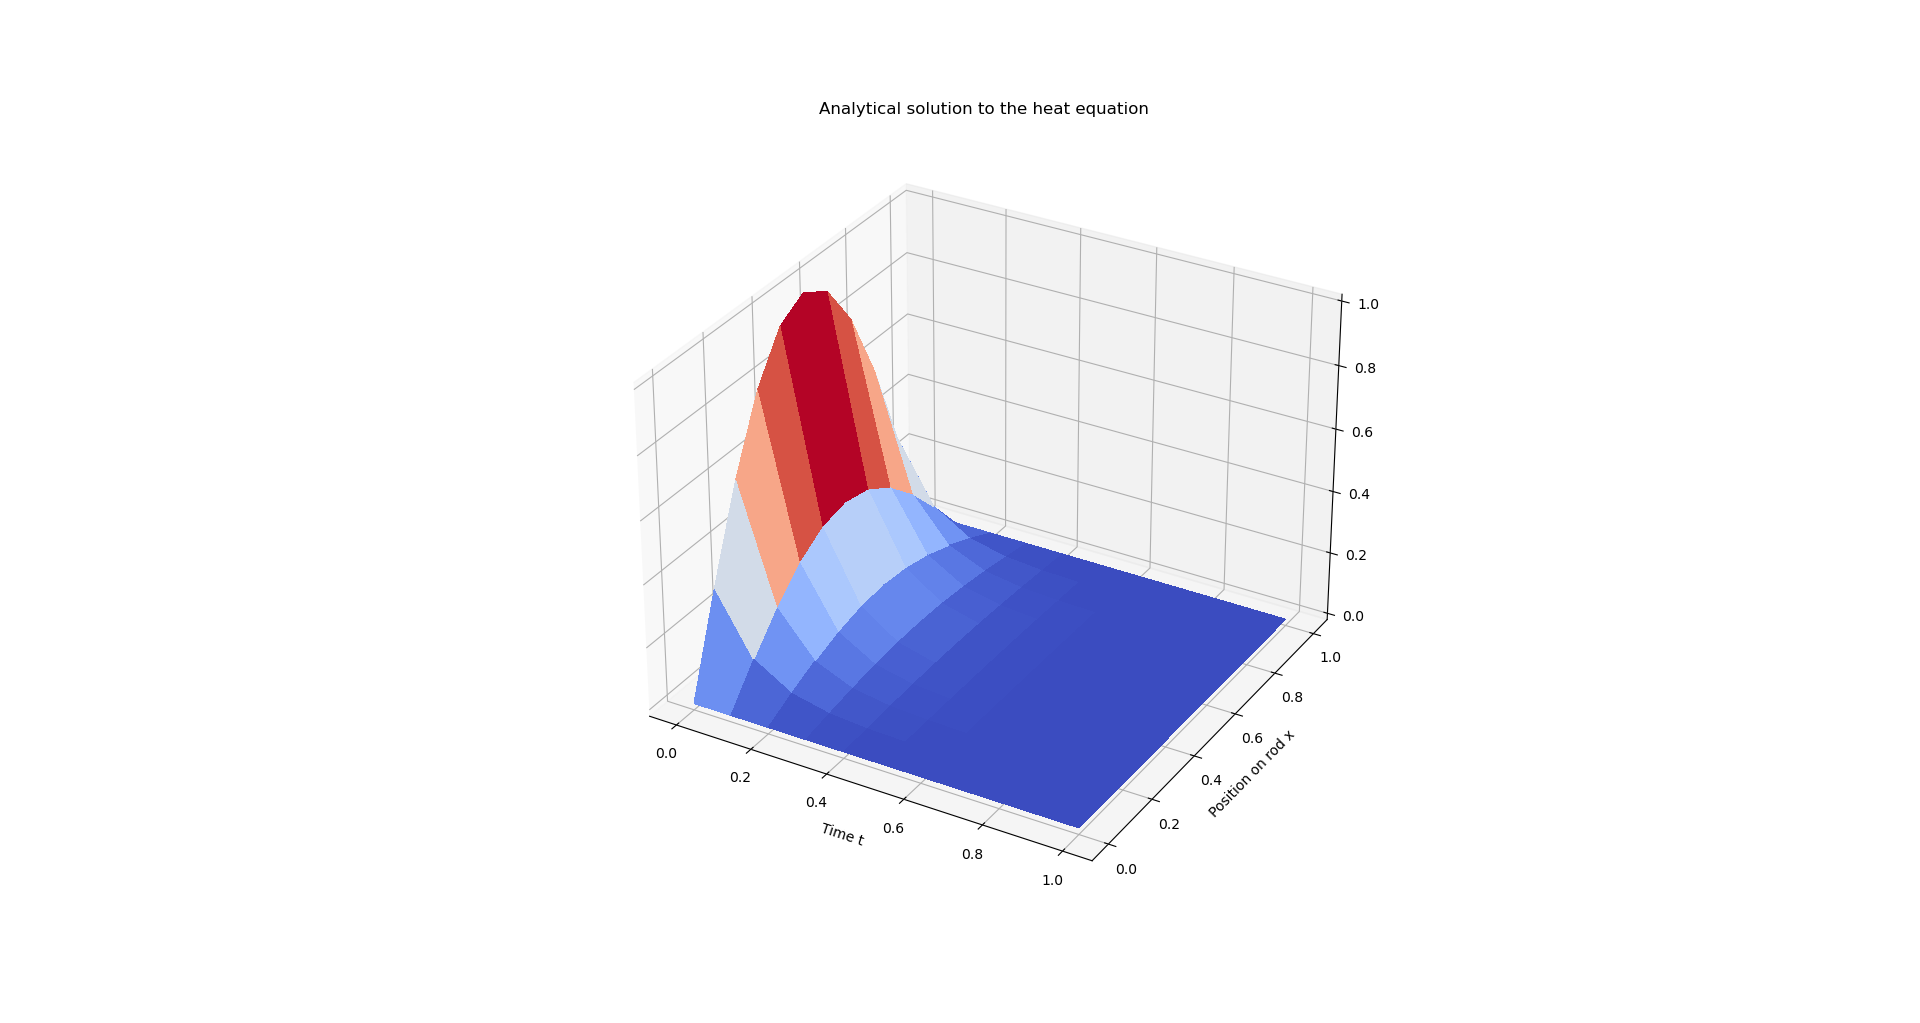
\includegraphics[width = 1\linewidth]{C:/Users/Sander/Documents/GitHub/FYS-STK4155/Project3/Report/Figures/3dHeat_ana.PNG}
\caption{\label{fig:3dHeatAna} Heat distribution for the rod as function of space and time for the analytical implementation.}
\end{figure}

\begin{figure}[H]
\centering
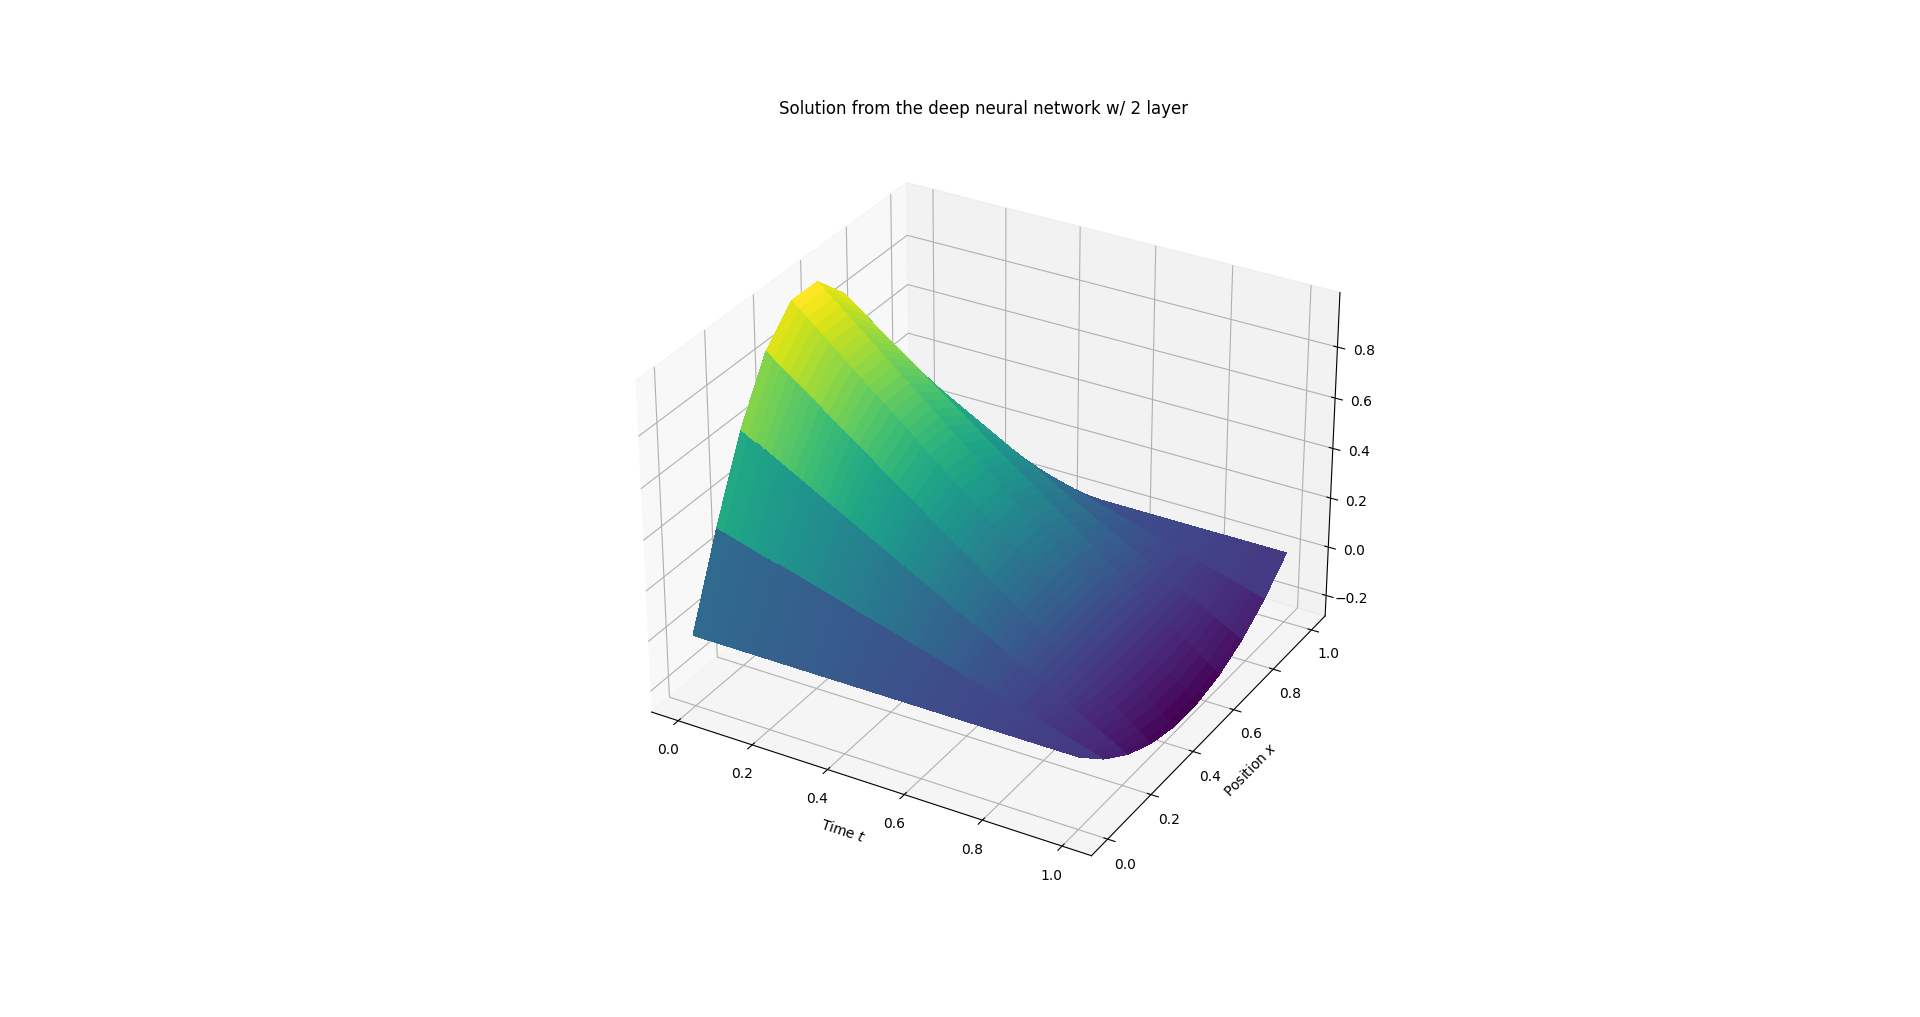
\includegraphics[width = 1\linewidth]{C:/Users/Sander/Documents/GitHub/FYS-STK4155/Project3/Report/Figures/3dHeat_NN.PNG}
\caption{\label{fig:3dHeatNN} Heat distribution for the rod as function of space and time for the neural network implementation.}
\end{figure}

\noindent One can observe that the two implementations in figures \ref{fig:3dHeatAna} and \ref{fig:3dHeatNN} are pretty similar. In order to get a better comparison, we can plot the heat distribution at constant times $t = 0$ (initial heat), $t = 0.5$ and $t = 1$ just like before.

\begin{figure}[H]
\centering
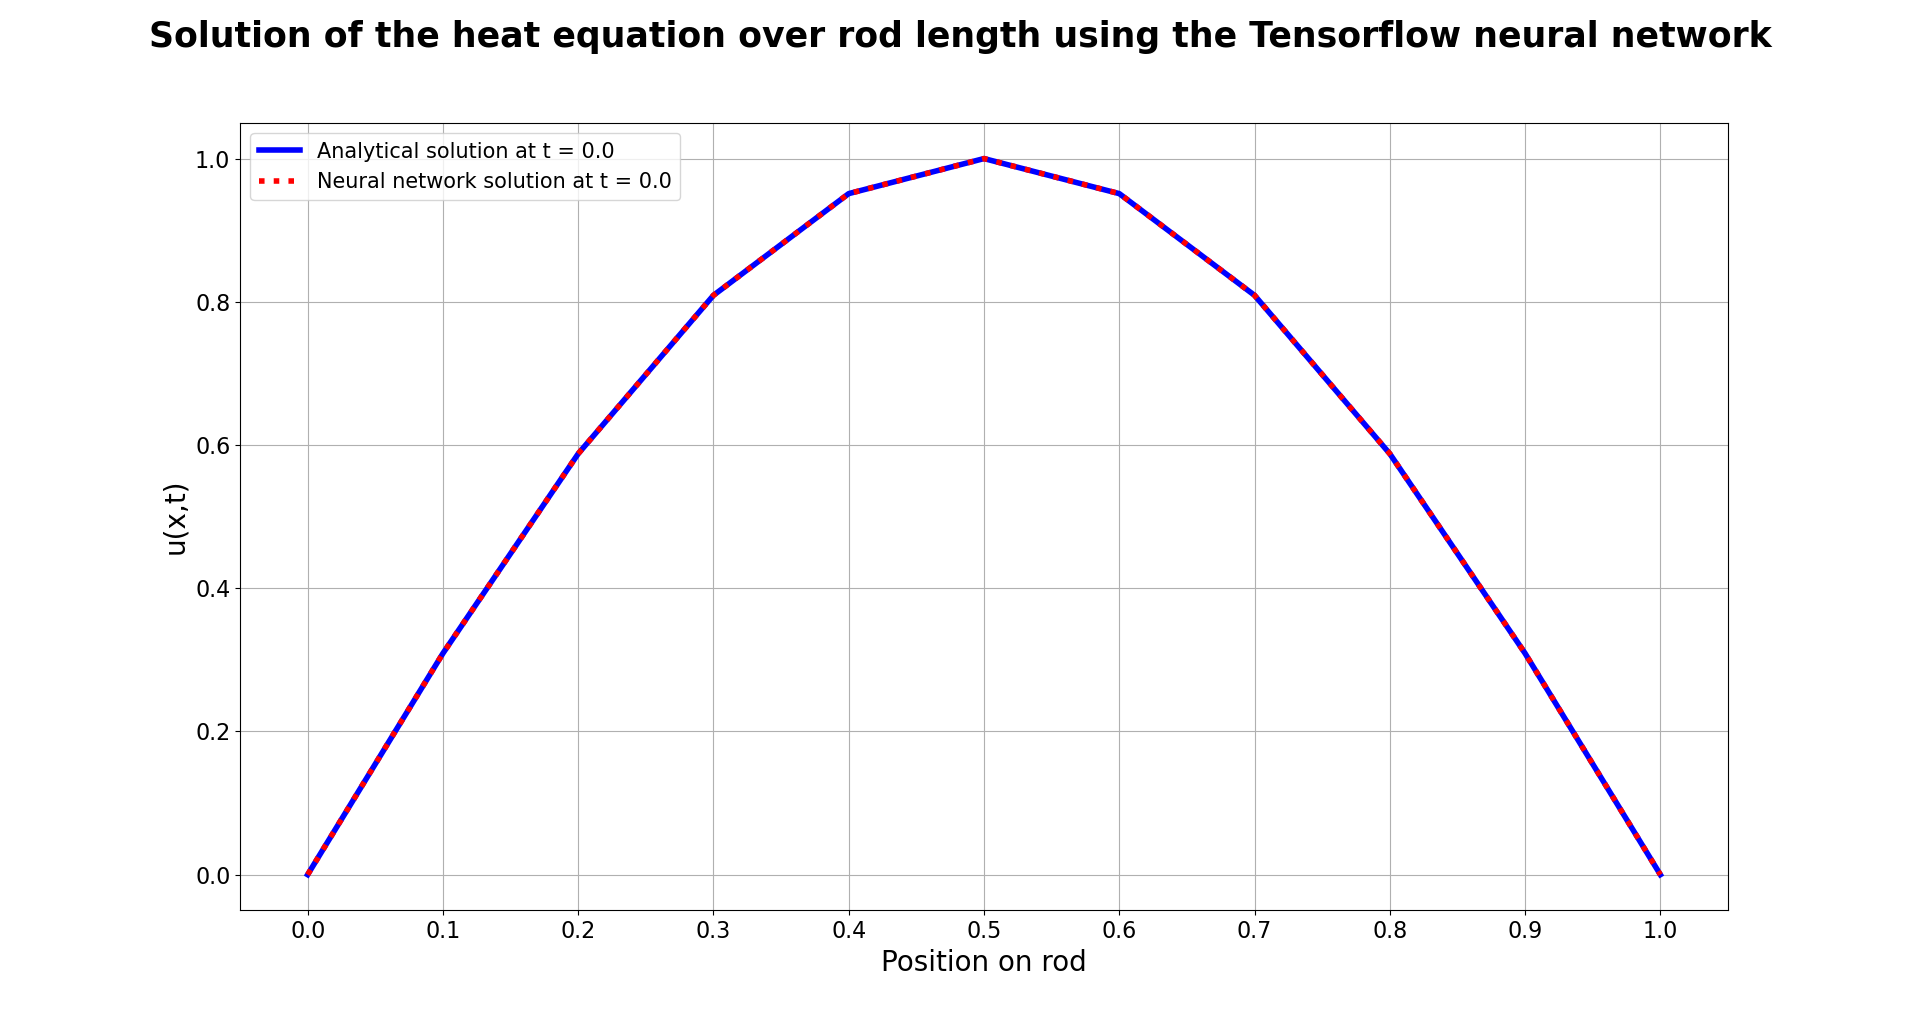
\includegraphics[width = 1\linewidth]{C:/Users/Sander/Documents/GitHub/FYS-STK4155/Project3/Report/Figures/Heat_TF_t0.PNG}
\caption{\label{fig:rodHeatTF0} Heat distribution within the rod for both analytical (blue) and neural network implementations (red). The heat is measured at $t = 0$ using the parameters of table \ref{tab:NNparams}.}
\end{figure}

\begin{figure}[H]
\centering
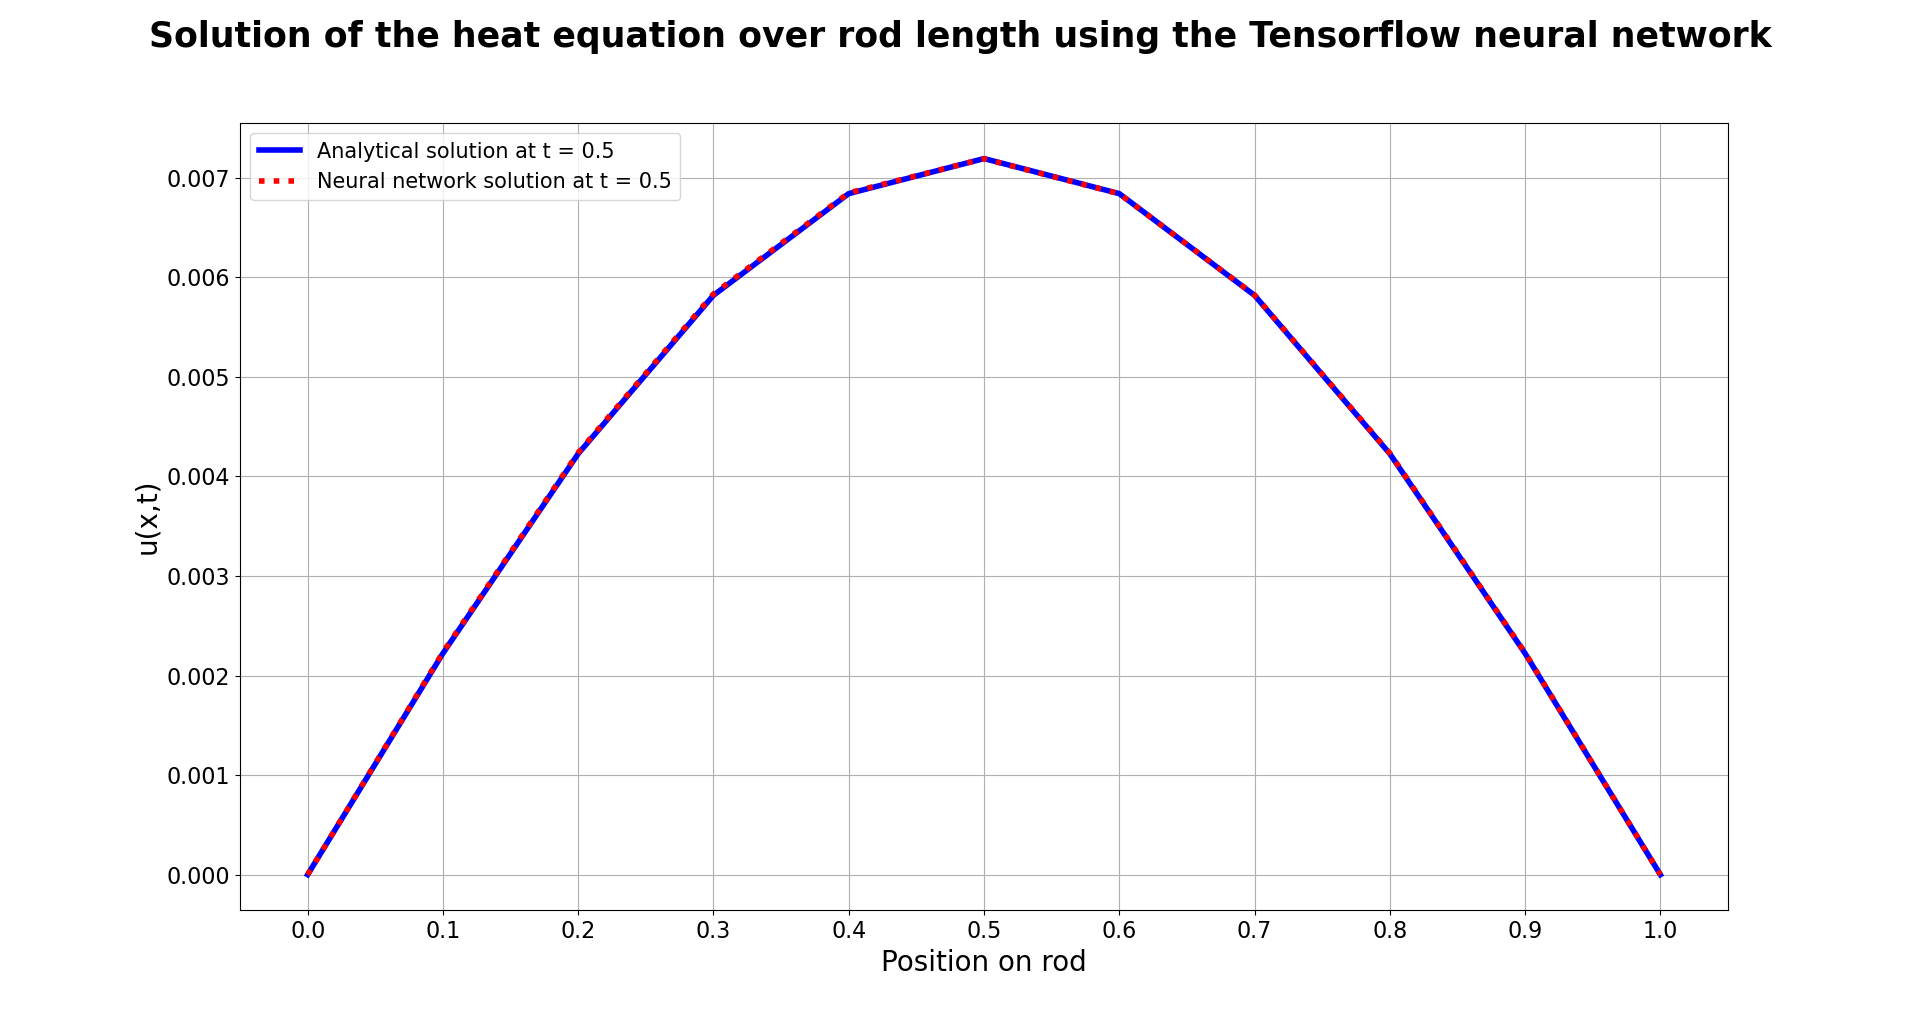
\includegraphics[width = 1\linewidth]{C:/Users/Sander/Documents/GitHub/FYS-STK4155/Project3/Report/Figures/Heat_TF_t05.PNG}
\caption{\label{fig:rodHeatTF05} Heat distribution within the rod for both analytical (blue) and neural network implementations (red). The heat is measured at $t = 0.5$ using the parameters of table \ref{tab:NNparams}.}
\end{figure}

\begin{figure}[H]
\centering
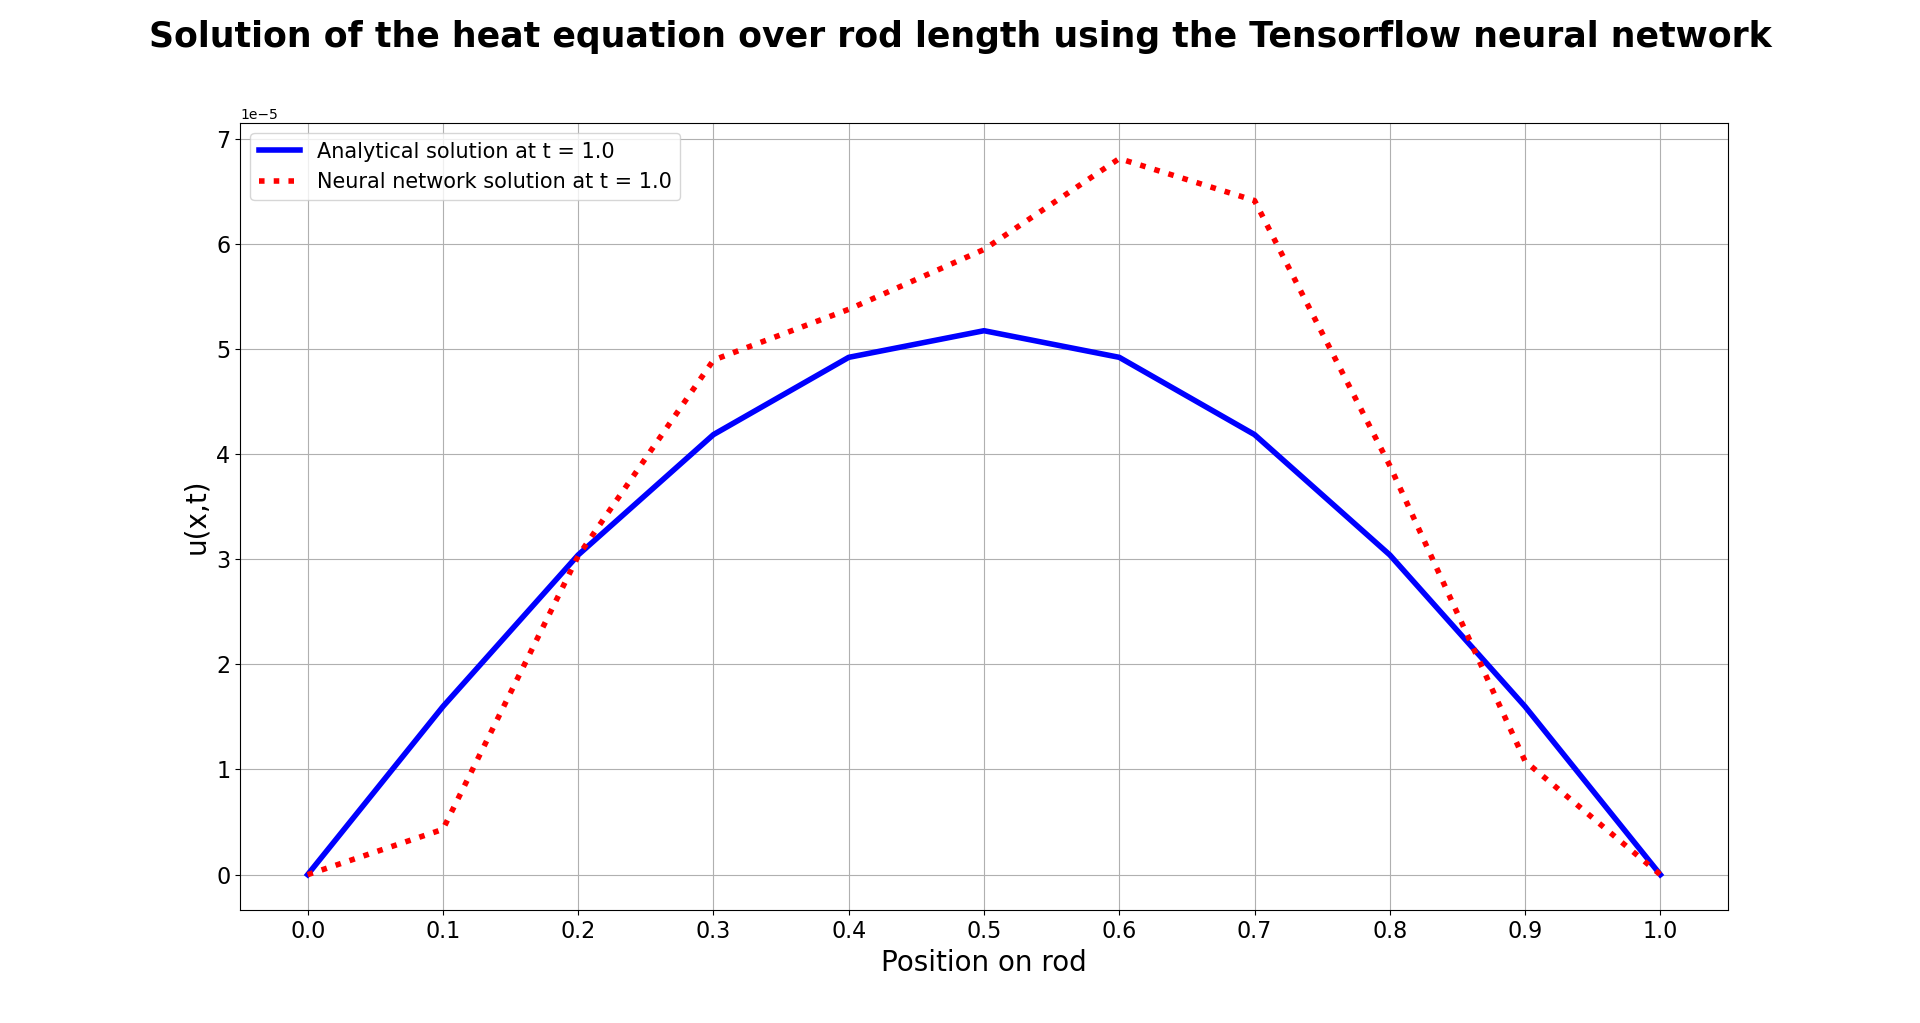
\includegraphics[width = 1\linewidth]{C:/Users/Sander/Documents/GitHub/FYS-STK4155/Project3/Report/Figures/Heat_TF_t1.PNG}
\caption{\label{fig:rodHeatTF1} Heat distribution within the rod for both analytical (blue) and neural network implementations (red). The heat is measured at $t = 1$ using the parameters of table \ref{tab:NNparams}.}
\end{figure}

\noindent One can observe that the initial heat distribution in figure \ref{fig:rodHeatTF0} is equal for the analytical and neural network implementations. After $0.5$ seconds however, the two implementations starts to deviate slightly. At $t = 1$ the two implementations are essentially zero, but the neural network still maintain the shape of the previous heat distributions. This was a recurring problem with the neural network implementation regardless of input parameters. However, since the error is very small, the result is deemed acceptable. 

\newpage

\begin{center}
\Large{\textbf{Exercise e): a}}
\end{center}

\noindent a

\newpage

\begin{center}
\Large{\textbf{Conclusion}}
\end{center}

\noindent a

\newpage

\begin{center}
\Large{\textbf{Future work}}
\end{center}

\noindent a

\newpage

\begin{center}
\Large{\textbf{References}}
\end{center}

\begin{itemize}
  \item Hancock, M. J., 2006, \emph{The 1-D Heat Equation, Linear Partial Differential Equations}, page 5, Available from \href{{https://ocw.mit.edu/courses/mathematics/18-303-linear-partial-differential-equations-fall-2006/lecture-notes/heateqni.pdf}}{\nolinkurl{https://ocw.mit.edu/courses/mathematics/18-303-linear-partial-differential-equations-fall-2006/lecture-notes/heateqni.pdf}}
  \item Kingma, D. P., Ba, J. L., 2014 \emph{Adam: A Method for Stochastic Optimization}, pp 1, arXiv:1412.6980v9
\end{itemize}

\end{document}
